\documentclass[a4paper,fleqn,12pt]{cas-sc}

\usepackage[authoryear]{natbib}
\usepackage{tcolorbox}
\usepackage{graphicx}
\usepackage{textcomp}

\usepackage{amsfonts} % 显式加载字体
\DeclareMathAlphabet{\mathbb}{U}{msb}{m}{n}

\usepackage[linesnumbered, ruled]{algorithm2e}
\SetKwRepeat{Do}{do}{while}%
\newcommand\mycommfont[1]{\footnotesize\ttfamily\textcolor{blue}{#1}}
\SetCommentSty{mycommfont}

\usepackage{amssymb} % for empty set
\usepackage{booktabs}
\usepackage{tabularx}
\usepackage{array}
\usepackage{float}
\usepackage[flushleft]{threeparttable}
\usepackage{tabularray} % for better
\usepackage[subsection]{placeins}

\frenchspacing % for consistent spacing between sentences

\newcommand{\killpunct}[1]{} % for reference, remove the comma in the reference of Proceeding

\usepackage{caption}
\DeclareCaptionFont{singlespacing}{\singlespacing}
\captionsetup{font=singlespacing}

\usepackage{subcaption}

\usepackage{tabularray}

\usepackage{etoolbox}

% Modify font size of the bibliography
\apptocmd{\thebibliography}{\fontsize{10}{14}\selectfont}{}{}

\usepackage{capt-of}

\usepackage{lineno}

\usepackage{titlesec}
\titleformat*{\section}{\fontsize{12}{20}\selectfont\bfseries}

\usepackage{titlesec}
\titleformat*{\subsection}{\fontsize{12}{20}\selectfont\bfseries}

\SetKwInput{KwData}{Input}
\SetKwInput{KwResult}{Output}

\usepackage{diagbox}
% centering figure and table captions

%%%Author macros
\def\tsc#1{\csdef{#1}{\textsc{\lowercase{#1}}\xspace}}
\tsc{WGM}
\tsc{QE}
\tsc{EP}
\tsc{PMS}
\tsc{BEC}
\tsc{DE}
%%%

\begin{document}
\let\WriteBookmarks\relax
\def\floatpagepagefraction{1}
\def\textpagefraction{.001}
\shorttitle{Preprint submitted to \textit{Elsevier journal}}
% \shortauthors{Lei et~al.}
%\begin{frontmatter}

\title [mode = title]{Transit Program Impact Evaluation: A Social Media Data Mining and Causal Inference Framework} 

\author[1]{Da Lei}[%
]

\address[1]{Department of Geography and Resource Management, The Chinese University of Hong Kong, Hong Kong, China}
\address[2]{School of Humanities and Social Science, The Chinese University of Hong Kong, Shenzhen, China}


\author[1]{Sylvia He}[\%
]
\cormark[1]

\author[2]{Shuli Luo}[\%
]

\cortext[cor1]{Corresponding author}


\begin{abstract}
Passenger feedback is a critical indicator for evaluating the effectiveness of transit improvement programs, with social media emerging as an important data source. This study develops a novel framework by linking unstructured social media posts to specific transit improvement programs, which are corresponding to our pre-defined transit service quality dimensions. We first conduct a text matching to align passenger feedback with program objectives, which includes a Latent Dirichlet Allocation (LDA) and Term Frequency-Inverse Document Frequency (TF-IDF) to identify latent themes from social media posts and a neural embedding for semantic matching. The matched data enables us to evaluate and quantify program impacts. Specifically, we begin by employing Interrupted Time Series Analysis (ITSA) to quantify the sentiment trends before and after program implementation, distinguishing short-term impacts from sustained improvements while controlling for seasonal patterns and temporal autocorrelation. The proposed framework is validated in a case study using 88,253 Weibo posts related to Shenzhen Metro services collected between January 2019 and July 2023. Results reveal statistically significant differences and shifts in public opinion in the targeted dimensions of several service improvement programs. Our approach can be applied to transit program evaluation in other cities beyond our case study area. This is 
\end{abstract}

\begin{keywords}
 \sep social media data \sep project impact evaluation \sep transit service quality
\end{keywords}


\maketitle
\setlength{\parindent}{15pt}
\setlength{\parskip}{0.1in}
\linenumbers

\section{Introduction}\label{sec:introduction}

Public transportation plays a crucial role in urban mobility systems, offering an essential service that contributes to sustainable development goals by reducing congestion, air pollution, and greenhouse gas emissions \citep{stjernborg2016role, mead2021road}. Despite these benefits, transit agencies worldwide face persistent challenges in attracting and retaining riders, particularly in competing with private vehicles and emerging mobility services \citep{beirAo2007understanding}. To address this issue, transit operators continuously implement various service improvement programs, ranging from technological upgrades and infrastructure renovations to policy changes and customer service enhancements \citep{luong2015public, fraser2024using}. 

Evaluating the effectiveness of these transit improvement programs is fundamental to the strategic planning and operational management of public transportation systems. Traditional evaluation methods rely heavily on performance metrics such as ridership counts, on-time performance, and customer satisfaction surveys \citep{nathanail2008measuring, eboli2011methodology}. While these metrics provide valuable insights, they often fail to capture the nuanced perspectives and real-time feedback of transit users \citep{collins2013novel}. This limitation is particularly significant given that passenger perceptions and experiences directly influence their decision to choose public transit over other modes of transportation \citep{friman2001frequency, morton2016customer}.

With the proliferation of social media platforms and the increasing willingness of the public to share their experiences online, a vast reservoir of user-generated content related to public transit has become available \citep{golder2011diurnal, kaplan2010users}. This data represents an untapped resource for transit agencies seeking to understand passenger sentiments and evaluate the impacts of their service improvement initiatives \citep{el2019linking, zhang2023changes}. Social media data offers several advantages over traditional data sources: it provides real-time feedback, captures spontaneous and unfiltered user opinions, and potentially reaches a broader and more diverse audience than conventional surveys \citep{tasse2014using, haghighi2018using}.

Recent research has begun to explore the potential of social media data in various aspects of transportation planning and analysis. Studies have demonstrated the utility of Twitter data for detecting traffic incidents \citep{fu2015social}, analyzing public opinions on transit services \citep{luong2015public, collins2013novel}, and evaluating public response to transportation policies \citep{chakraborty2019public}. However, these studies often focus on general sentiment analysis without specifically linking social media content to particular transit improvement programs or interventions \citep{ali2017fuzzy, ingvardson2019relationship}. This gap limits the practical utility of social media analytics for program evaluation and decision-making processes in transit agencies. Moreover, the methodological approaches for processing and analyzing social media data in the context of transit evaluation remain relatively underdeveloped. Existing studies often rely on simple keyword searches and basic sentiment scoring, which may not adequately capture the complexity and contextual nuances of passenger feedback \citep{houston2015public, kamga2023utilizing}. There is a need for more sophisticated frameworks that can effectively extract relevant information from unstructured social media posts and link them to specific dimensions of transit service quality \citep{haghighi2018using}.

To address these limitations, this study proposes a novel framework that combines advanced text mining techniques with causal inference methods to evaluate the impact of transit improvement programs using social media data. The framework consists of three main components: (1) a text matching process that aligns passenger feedback from social media with specific transit improvement programs and service quality dimensions; (2) an Interrupted Time Series Analysis (ITSA) that quantifies changes in passenger sentiments before and after program implementation; and (3) a set of statistical tests to assess the significance and sustainability of program impacts. The text matching process employs Latent Dirichlet Allocation (LDA) for topic modeling and Term Frequency-Inverse Document Frequency (TF-IDF) for feature extraction, followed by neural embeddings for semantic matching. This combination of techniques allows for the identification of relevant social media posts that reflect passenger experiences related to specific transit improvement initiatives, even when the posts do not explicitly mention the program names or use standard terminology \citep{blei2003latent, lopez2016interrupted}. The ITSA method is particularly well-suited for evaluating the impact of interventions that have been implemented at clearly defined points in time \citep{wagner2002segmented, lopez2016interrupted}. By modeling the trends of passenger sentiments before and after program implementation, ITSA can distinguish between short-term fluctuations and sustained improvements, while controlling for confounding factors such as seasonal patterns and temporal autocorrelation \citep{schaffer2021interrupted, koppel2023disentangling}.

To validate our framework, we apply it to a case study of Shenzhen Metro in China, using 88,253 Weibo posts collected from January 2019 to July 2023. The case study focuses on several service improvement programs implemented by Shenzhen Metro during this period, covering different dimensions of transit service quality such as comfort, reliability, safety, and information provision. The results demonstrate the effectiveness of our approach in capturing significant changes in passenger sentiments following the implementation of these programs and provide insights into the varying impacts across different service quality dimensions. The contributions of this study are threefold. First, we develop a novel methodological framework that bridges the gap between unstructured social media data and structured program evaluation, enabling transit agencies to leverage the wealth of information available on social media platforms. Second, we demonstrate the application of ITSA in the context of transit program evaluation, providing a robust statistical approach to quantify program impacts while accounting for various confounding factors. Third, we offer empirical evidence on the effectiveness of several transit improvement programs in Shenzhen Metro, contributing to the growing body of knowledge on best practices in public transportation management.

The remainder of this paper is organized as follows. Section 2 reviews the relevant literature on transit service quality evaluation, social media analytics in transportation, and causal inference methods for program impact assessment. Section 3 describes the methodology in detail, including the text matching process, ITSA model specification, and statistical testing procedures. Section 4 presents the case study of Shenzhen Metro, detailing the data collection, program descriptions, and analysis results. Finally, Section 5 concludes with a discussion of the implications, limitations, and future directions of this research.

\section{Literature Review}\label{sec:liter}

\subsection{Transit Service Quality Assessment Frameworks}
The evaluation of public transportation service quality has been a subject of extensive research over the past decades. Traditional assessment frameworks have typically focused on objective performance indicators and subjective user perceptions, often captured through structured surveys and predefined metrics \citep{de2013composite, eboli2011methodology}. \cite{nathanail2008measuring} proposed a comprehensive framework incorporating safety, reliability, cleanliness, comfort, servicing, passenger information, and accessibility as key dimensions of service quality. Similarly, \cite{dell2011public} developed a multi-criteria approach that balances technical efficiency with service effectiveness and societal impact.

The European Committee for Standardization established a widely adopted framework (EN 13816) that defines eight quality categories: availability, accessibility, information, time, customer care, comfort, security, and environmental impact \citep{europeancommittee2002}, providing a standardized approach to transit service evaluation. Building on this foundation, \cite{de2018novel} introduced an enhanced methodology that incorporates both objective measures and subjective assessments to create a more balanced evaluation framework. In the North American context, the Transit Capacity and Quality of Service Manual \citep{kittelson2003transit} offers a structured approach focusing on availability (frequency, service span, and coverage) and comfort/convenience (passenger load, reliability, and transit-auto travel time). This framework has been widely adopted by transit agencies across the United States and Canada, although \cite{morton2016perceptions} argues that it may not fully capture the nuanced aspects of user experience.

Recent research has emphasized the importance of context-specific evaluation, recognizing that service quality perceptions vary across different urban environments, demographic groups, and cultural contexts \citep{dell2018methodology, diab2017transit}. \cite{zhao2013web} highlighted how different user segments prioritize different service attributes, suggesting that evaluation frameworks should be adaptable to local conditions and user expectations. Similarly, \cite{wang2020analyzing} demonstrated that service quality perceptions are influenced by both objective service attributes and subjective user characteristics, emphasizing the need for more nuanced assessment approaches.

Despite these advancements, traditional evaluation methods continue to face limitations in terms of cost, timeliness, comprehensiveness, and potential response biases \citep{hensher2003service, de2018novel}. Survey-based approaches often capture only a snapshot of user perceptions, potentially missing temporal variations in service quality and user experiences \citep{chang2013exploring}. Additionally, predetermined evaluation criteria may not always align with the aspects of service that matter most to users in specific contexts \citep{van2019influence, tyrinopoulos2008public}.

\subsection{Social Media Data in Transportation Research}
The proliferation of social media platforms has created new opportunities for accessing large volumes of unsolicited public opinion on various aspects of urban life, including transportation services \citep{collins2013social, schweitzer2012social}. Unlike structured surveys, social media offers spontaneous, real-time expressions of user experiences, potentially capturing dimensions of service quality that might not be included in predetermined evaluation frameworks \citep{gal2014traveling, luong2015mining}.

Early applications of social media data in transportation research focused primarily on event detection and traffic monitoring \citep{steiger2015twitter, yuan2016discovering}. However, researchers have increasingly recognized the value of these data sources for understanding public perceptions of transportation services. \cite{collins2013social} analyzed Twitter data to identify patterns in public discourse about public transportation in Chicago, demonstrating the potential of social media for capturing temporal and spatial variations in user experiences. Similarly, \cite{schweitzer2012social} examined tweets related to public transit agencies in the United States, finding significant associations between sentiment expressed on Twitter and objective service quality metrics.

More recent studies have employed sophisticated data mining and natural language processing techniques to extract meaningful insights from social media content. \cite{zhang2019examining} developed a framework for analyzing geo-tagged tweets to understand spatial patterns in sentiment toward transit services in New York City. \cite{wang2020mining} employed topic modeling and sentiment analysis to identify key themes in public discourse about high-speed rail in China, revealing insights that would be difficult to capture through traditional surveys. The integration of geo-location data with social media content has further enhanced the value of these platforms for transportation research. \cite{rashidi2017exploring} demonstrated how geo-tagged social media data can be used to analyze travel behavior and mode choice, while \cite{maeda2019transportation} developed a methodology for extracting transportation-related information from location-based social media to support infrastructure planning.

Despite these advancements, researchers have identified several challenges in using social media data for transportation analysis. \cite{efthymiou2013use} highlighted concerns about sample representativeness, noting that social media users may not reflect the broader population of transit riders. \cite{nguyen2016transportation} discussed issues related to data quality, including the presence of spam, irrelevant content, and varying levels of linguistic complexity. Additionally, \cite{tse2018social} emphasized the challenges of accurately interpreting sentiment and context in short, informal social media posts.

\subsection{Causal Inference in Transportation Program Evaluation}
Establishing causal relationships between transportation interventions and observed outcomes represents a significant methodological challenge in program evaluation \citep{karner2016transportation, hong2020causal}. Traditional before-after comparisons often fail to account for secular trends, seasonality, and confounding factors that may influence the observed changes independently of the intervention \citep{lechner2011estimation, imbens2015causal}.

Quasi-experimental designs have emerged as valuable approaches for strengthening causal inference in transportation program evaluation. Among these, interrupted time series (ITS) analysis has gained prominence as a robust method for assessing the impact of interventions when randomization is not feasible \citep{bernal2017interrupted, lopez2017interrupted}. The ITS approach examines the trajectory of an outcome measure before and after an intervention, accounting for pre-existing trends to isolate the effect of the intervention \citep{wagner2002segmented, bernal2016methodological}. \cite{kontopantelis2015regression} demonstrated the application of ITS analysis in evaluating policy interventions, highlighting its ability to control for time-varying confounders and detect both immediate and gradual effects. In the transportation context, \cite{morrison2018impact} employed ITS analysis to evaluate the impact of a new light rail line on traffic congestion, distinguishing the intervention effect from seasonal and long-term trends. Similarly, \cite{baek2016using} utilized this approach to assess the effectiveness of transit service improvements in increasing ridership, controlling for external factors such as fuel prices and economic conditions.

Advanced causal inference methods, such as difference-in-differences (DiD) and synthetic control methods, have also been applied in transportation program evaluation. \cite{hong2020causal} employed a DiD approach to evaluate the impact of transit-oriented development on travel behavior, comparing treated and control areas while accounting for time-invariant unobserved characteristics. \cite{ye2020causal} developed a synthetic control framework for assessing the impact of transportation infrastructure investments on economic outcomes, creating a counterfactual scenario from a weighted combination of control units.

The integration of machine learning with causal inference has opened new avenues for transportation program evaluation. \cite{athey2017state} discussed how machine learning techniques can enhance causal inference by improving the estimation of treatment effects and addressing high-dimensional confounding. \cite{spirtes2016causal} presented a framework for using causal discovery algorithms to identify potential causal relationships from observational data, which could be valuable for understanding complex interactions in transportation systems.

Despite these methodological advancements, challenges remain in applying causal inference to transportation program evaluation. \cite{imbens2015causal} highlighted the importance of addressing potential violations of key assumptions, such as the stable unit treatment value assumption (SUTVA) and the parallel trends assumption in DiD designs. \cite{angrist2008mostly} emphasized the need for careful consideration of instrumental variables and potential selection biases in natural experiments. Additionally, \cite{pearl2009causality} stressed the importance of explicit causal modeling to clarify assumptions and enhance the interpretability of results.

\subsection{Integrated Approaches for Transit Service Evaluation}
Recent research has increasingly focused on integrating multiple data sources and methodologies to create more comprehensive approaches to transit service evaluation \citep{tse2018social, ma2018integrated}. These integrated approaches aim to leverage the strengths of different data types while mitigating their respective limitations.

\cite{zhao2013web} demonstrated how web-based surveys could be combined with traditional intercept surveys to reach a broader population of transit users and non-users, providing a more comprehensive understanding of service perceptions. Building on this work, \cite{barbosa2017combining} developed a framework that integrates passenger surveys with objective performance metrics and operational data to create a multi-dimensional evaluation of transit service quality. The combination of social media data with traditional evaluation methods has emerged as a particularly promising approach. \cite{collins2013social} proposed a framework for triangulating insights from social media analysis with passenger surveys and operational metrics, demonstrating how these complementary data sources can provide a more nuanced understanding of service quality. Similarly, \cite{wu2020integrated} developed a methodology that combines sentiment analysis of social media content with passenger flow data to identify critical service issues and prioritize improvements.

Advanced statistical and computational methods have facilitated the integration of diverse data types for transit evaluation. \cite{zhang2018analytics} employed machine learning techniques to integrate structured operational data with unstructured text data from social media, creating a unified framework for service quality assessment. \cite{jin2020deep} demonstrated how deep learning approaches can be used to extract meaningful patterns from heterogeneous data sources, including social media, smart card records, and vehicle tracking data. The spatial dimension of transit service evaluation has also been enhanced through integrated approaches. \cite{gal2014traveling} combined geo-tagged social media data with spatial analysis techniques to identify geographic patterns in service perceptions, allowing for more targeted improvement strategies. \cite{wang2020analyzing} integrated spatial accessibility measures with sentiment analysis of social media content to examine the relationship between physical access to transit and user satisfaction.

Despite the potential of integrated approaches, several challenges remain in their implementation. \cite{tse2018social} highlighted issues related to data integration and compatibility, noting that different data sources may have varying temporal and spatial resolutions. \cite{nguyen2016transportation} discussed methodological challenges in combining quantitative and qualitative data types, emphasizing the need for robust analytical frameworks. Additionally, \cite{zhang2019examining} pointed out practical challenges related to data access, privacy concerns, and technical requirements for implementing integrated evaluation approaches.

\subsection{Research Gaps and Contributions}
The literature reveals several important gaps in current approaches to transit service evaluation. First, while social media data has been increasingly used in transportation research, methodologically rigorous frameworks for leveraging these data sources for program evaluation remain underdeveloped \citep{schweitzer2012social, zhang2019examining}. Second, causal inference methods have been applied to transportation interventions, but their integration with social media data analysis is still in its infancy \citep{hong2020causal, ye2020causal}. Third, existing studies often focus on either sentiment analysis or thematic content extraction from social media, but rarely combine these approaches to create comprehensive service quality indicators \citep{collins2013social, luong2015mining}.

This research addresses these gaps by developing an integrated framework that combines advanced social media data mining techniques with robust causal inference methodologies. The framework leverages natural language processing and machine learning to extract both sentiment and thematic content from social media posts, creating a multi-dimensional representation of public perceptions of transit services. It then applies interrupted time series analysis to establish causal relationships between service improvements and changes in these perceptions, accounting for pre-existing trends and potential confounding factors.

By bridging the gap between data-rich social media platforms and methodologically rigorous causal inference approaches, this research offers transit agencies a novel, cost-effective method for evaluating service improvements that captures authentic public feedback while maintaining analytical rigor. The demonstration of this framework through a real-world case study provides empirical evidence of its practical utility and highlights its potential for enhancing evidence-based decision-making in transit planning and management.

\section{Methodology}\label{sec:Methodology}

This section presents our methodological framework for evaluating transit improvement programs using social media data. The framework integrates advanced natural language processing (NLP) techniques with robust causal inference methods to systematically analyze how transit improvement programs influence passenger sentiment. As illustrated in Figure \ref{fig:methodology_framework}, our approach consists of three main components: (1) data preprocessing and semantic matching, (2) sentiment analysis and aggregation, and (3) impact evaluation using interrupted time series analysis.

\subsection{Data Preprocessing and Semantic Matching}

\subsubsection{Latent Dirichlet Allocation for Topic Discovery}

The first step in our framework involves processing unstructured social media posts to identify latent themes relevant to transit service quality. We employ Latent Dirichlet Allocation (LDA) \citep{blei2003latent}, a probabilistic topic modeling technique that discovers hidden thematic structures within text data. LDA models each document as a mixture of topics, where each topic is characterized by a distribution over words.

For preprocessing, we first remove URLs, special characters, and numbers from the text, then segment Chinese text using Jieba \citep{sun2012jieba}, a Chinese text segmentation library. We eliminate stopwords and short words (typically single characters), as they convey minimal semantic meaning. To improve the segmentation quality for transit-specific content, we augment the Jieba dictionary with domain-relevant terms such as metro station names.

The LDA model is formally defined as:

\begin{align}
p(\theta, \mathbf{z}, \mathbf{w} | \alpha, \beta) = p(\theta | \alpha) \prod_{n=1}^{N} p(z_n | \theta) p(w_n | z_n, \beta)
\end{align}

where $\theta$ represents the document-topic distribution, $\mathbf{z}$ denotes the topic assignments, $\mathbf{w}$ represents the observed words, and $\alpha$ and $\beta$ are the hyperparameters for the Dirichlet priors on the document-topic and topic-word distributions, respectively.

To enhance model robustness, we optimize the LDA hyperparameters through multiple initializations with different random seeds, selecting the model with the lowest perplexity score. For our implementation, we set the number of topics $K = 15$, document-topic prior $\alpha = 0.05$, and topic-word prior $\beta = 0.005$, which we determined through empirical testing to provide interpretable topics while maintaining adequate discrimination between service quality dimensions.

\subsubsection{TF-IDF Feature Extraction}

After topic modeling, we employ Term Frequency-Inverse Document Frequency (TF-IDF) transformation to identify the most distinctive terms for each topic. The TF-IDF score for a term $t$ in document $d$ within corpus $D$ is computed as:

\begin{align}
\text{TF-IDF}(t, d, D) = \text{TF}(t, d) \times \text{IDF}(t, D)
\end{align}

where $\text{TF}(t, d)$ is the frequency of term $t$ in document $d$, and $\text{IDF}(t, D)$ is calculated as:

\begin{align}
\text{IDF}(t, D) = \log\frac{|D|}{|\{d \in D: t \in d\}|}
\end{align}

This transformation assigns higher weights to terms that are frequent in a specific document but rare across the corpus, which helps identify the most characteristic words for each topic. We apply TF-IDF transformation to the word-document matrix before fitting the LDA model, which helps improve topic coherence and interpretability \citep{ming2014understanding}.

\subsubsection{Neural Embedding for Semantic Matching}

To connect passenger feedback with specific transit improvement programs, we implement a semantic matching approach using neural embeddings. Specifically, we utilize the multilingual MiniLM-L12-v2 model from the sentence-transformers framework \citep{reimers2019sentence}, which maps text into a dense 384-dimensional vector space where semantically similar texts have high cosine similarity.

For each service improvement program, we create a document that describes its objectives and features, then compute the embedding vector for this description. Similarly, we compute embedding vectors for each processed social media post. The semantic similarity between a program $p$ and a post $s$ is calculated as:

\begin{align}
\text{sim}(p, s) = \frac{\mathbf{v}_p \cdot \mathbf{v}_s}{||\mathbf{v}_p|| \cdot ||\mathbf{v}_s||}
\end{align}

where $\mathbf{v}_p$ and $\mathbf{v}_s$ are the embedding vectors for the program description and social media post, respectively. We establish a similarity threshold of 0.35 based on empirical testing, which balances precision and recall in matching relevant posts to programs. Posts exceeding this threshold are considered relevant to the corresponding program and included in the subsequent analysis.

\subsection{Sentiment Analysis and Aggregation}

\subsubsection{Sentiment Analysis Approach}

Following semantic matching, we analyze the sentiment expressed in each relevant social media post. Given the specificity of transit-related terminology and the Chinese language context, we employ a domain-adapted sentiment analysis approach that combines lexicon-based methods with machine learning classification.

For each post, we compute a sentiment score in the range $[-1, 1]$, where $-1$ represents extremely negative sentiment, $0$ represents neutral sentiment, and $1$ represents extremely positive sentiment. The sentiment analysis process accounts for domain-specific terms, negation patterns, and intensifiers common in passenger feedback.

\subsubsection{Temporal Aggregation}

To prepare for time series analysis, we aggregate sentiment scores across different temporal granularities: daily, weekly, and monthly. For each program $p$ and time period $t$, we calculate:

\begin{align}
\bar{S}_{p,t} = \frac{1}{n_{p,t}} \sum_{i=1}^{n_{p,t}} s_i
\end{align}

where $\bar{S}_{p,t}$ is the mean sentiment score for program $p$ during time period $t$, $n_{p,t}$ is the number of posts relevant to program $p$ during period $t$, and $s_i$ is the sentiment score of post $i$.

We also calculate additional metrics for each time period, including sample size ($n_{p,t}$), which represents the number of posts relevant to program $p$ during period $t$; sentiment variance, which measures the variance of sentiment scores within each period; and sentiment distribution, which captures the proportion of positive, neutral, and negative posts—these aggregated metrics serve as the foundation for our causal impact analysis.

\subsection{Impact Evaluation Using Interrupted Time Series Analysis}

\subsubsection{Model Specification}

To quantify the impact of transit improvement programs on passenger sentiment, we employ Interrupted Time Series Analysis (ITSA), a quasi-experimental design that evaluates interventions by examining changes in time series data patterns before and after implementation \citep{bernal2017interrupted}. ITSA is particularly well-suited for our context as it can distinguish between immediate and gradual effects while controlling for pre-existing trends.

Our core ITSA model specification is:

\begin{align}
Y_t = \beta_0 + \beta_1 T_t + \beta_2 X_t + \beta_3 X_t T_t + \epsilon_t
\end{align}

where $Y_t$ represents the mean sentiment score at time $t$, $T_t$ indicates the time elapsed since the start of the study, $X_t$ is a dummy variable that distinguishes between pre-intervention ($X_t = 0$) and post-intervention periods ($X_t = 1$), $X_t T_t$ serves as an interaction term measuring time since the intervention occurred, and $\epsilon_t$ denotes the error term.

In this model, $\beta_0$ represents the baseline level, $\beta_1$ captures the pre-intervention trend, $\beta_2$ indicates the immediate change in level following intervention, and $\beta_3$ represents the change in trend after intervention.

\subsubsection{Addressing Time Series Complexities}

To handle the complexities inherent in time series data, we extend the basic ITSA model to account for:

\textbf{Autocorrelation:} We test for autocorrelation in the residuals using the Durbin-Watson statistic and incorporate autoregressive (AR) terms when necessary:

\begin{align}
Y_t = \beta_0 + \beta_1 T_t + \beta_2 X_t + \beta_3 X_t T_t + \sum_{i=1}^{p} \phi_i Y_{t-i} + \epsilon_t
\end{align}

where $p$ is the order of the autoregressive process, and $\phi_i$ are the AR coefficients.

\textbf{Seasonal Patterns:} We incorporate seasonal components to account for cyclical variations in transit usage and social media activity:

\begin{align}
Y_t = \beta_0 + \beta_1 T_t + \beta_2 X_t + \beta_3 X_t T_t + \sum_{j=1}^{J} \gamma_j S_{j,t} + \epsilon_t
\end{align}

where $S_{j,t}$ are seasonal indicator variables, and $\gamma_j$ are the corresponding coefficients.

\textbf{Heteroskedasticity:} We implement robust standard errors to address potential heteroskedasticity in the variance of the error terms.

\subsubsection{Placebo Tests and Robustness Checks}

To strengthen causal inference, we conduct several robustness checks: performing placebo tests by artificially shifting the intervention point to different time periods (expecting the strongest effect at the true intervention point); controlling for variation in the number of social media posts across time periods by including sample size as a covariate; and testing alternative model specifications by varying parameters such as aggregation periods, semantic matching thresholds, and sentiment analysis approaches.


\section{Case study}\label{sec:CaseStudy}

\subsection{Overview of Shenzhen Metro System}

Shenzhen Metro, operated by Shenzhen Metro Group Co., Ltd., serves as the primary rapid transit system for Shenzhen, one of China's major metropolitan areas in Guangdong Province. Since its first line opened in 2004, the system has expanded significantly to accommodate the city's rapid growth and development. As of 2023, the network comprises 16 operational lines spanning approximately 530 kilometers with 345 stations, making it one of the largest and busiest metro systems in China \citep{chen2018demand}. The system serves a diverse population of over 13 million residents and handles an average daily ridership exceeding 7 million passengers \citep{li2022comparative}. As a technology hub often referred to as "China's Silicon Valley," Shenzhen has integrated numerous technological innovations into its metro operations, including digital payment systems, facial recognition technology, and AI-powered crowd management systems \citep{guo2019smart}. Shenzhen Metro has implemented various service improvement programs in recent years aimed at enhancing passenger experience across multiple dimensions of service quality. These improvements include technological innovations, infrastructure upgrades, policy changes, and customer service enhancements \citep{deng2021quality}. The evaluation of these programs presents an ideal context for applying our proposed framework, as it allows us to investigate how different types of service improvements affect passenger sentiment and experience.

\subsection{Data Collection and Processing}

\subsubsection{Social Media Data Source}

For our analysis, we collected 88,253 Weibo posts related to Shenzhen Metro services between January 2019 and July 2023. Weibo, often described as China's equivalent to Twitter, serves as a major platform for public expression and opinion sharing in China, with approximately 530 million monthly active users as of 2022 \citep{wang2022empirical}. This platform offers several advantages for transit program evaluation: it captures spontaneous, real-time passenger feedback outside the constraints of structured surveys, provides access to a larger and potentially more diverse sample of transit users, allows for the analysis of temporal patterns in public sentiment before and after program implementation, and contains rich contextual information, including user characteristics and interaction patterns.


The data collection process involved an API-based retrieval using keywords related to Shenzhen Metro, including the system's name in different variations (e.g., "深圳地铁", "深铁") and station names. We implemented comprehensive error handling and rate limiting to comply with platform policies while maximizing data quality.

\subsubsection{Data Preprocessing}

The collected Weibo posts underwent several preprocessing steps before analysis, as illustrated in Figure \ref{fig:preprocessing}. First, we removed URLs, special characters, and numbers from the text and segmented Chinese text using Jieba \citep{sun2012jieba}, a Chinese text segmentation library. To improve segmentation quality for transit-specific content, we augmented the dictionary with domain-relevant terms such as metro station names.

Following text cleaning, we applied Latent Dirichlet Allocation (LDA) to identify latent thematic structures within the corpus. The LDA model was optimized with a topic count of $K = 15$, document-topic prior $\alpha = 0.05$, and topic-word prior $\beta = 0.005$, determined through empirical testing to provide interpretable topics while maintaining adequate discrimination between service quality dimensions. To enhance topic coherence and interpretability, we employed Term Frequency-Inverse Document Frequency (TF-IDF) transformation, which assigns higher weights to terms that are frequent in specific documents but rare across the corpus. This approach helped distinguish the most characteristic words for each topic. The final step involved semantic matching between passenger feedback and specific transit improvement programs using neural embeddings. We utilized the multilingual MiniLM-L12-v2 model from the sentence-transformers framework \citep{reimers2019sentence}, which maps text into a dense 384-dimensional vector space. This allowed us to calculate semantic similarity between program descriptions and social media posts, with an empirically determined similarity threshold of 0.35 to balance precision and recall.

\subsection{Service Improvement Programs}

Our case study focused on six service improvement programs implemented by Shenzhen Metro between 2019 and 2023. These programs span different dimensions of transit service quality, including comfort, technology, convenience, affordability, and accessibility. Table \ref{tab:programs} provides an overview of these programs. Each program represents a distinct approach to service improvement.

\begin{table}[h]
\centering
\caption{Service Improvement Programs Analyzed in the Case Study}
\label{tab:programs}
\begin{tabular}{p{0.1\textwidth}p{0.47\textwidth}p{0.17\textwidth}p{0.18\textwidth}}
\hline
Program ID & Program Description & Service Dimension & Implementation Date \\
\hline
0 & Temperature Consistency Across Carriages (resolving temperature variation issue) & Comfort & August 2022 \\
1 & Smart Dynamic Map Display System & Information & October 2021 \\
4 & QR Code Scanning for Fare Payment & Convenience & March 2020 \\
5 & Renovation of Restrooms at 82 Stations & Amenities & June 2021 \\
15 & Mobile Nursing Rooms & Accessibility & September 2022 \\
22 & Fare Reduction & Affordability & January 2023 \\
\hline
\end{tabular}
\end{table}

\begin{table}[htbp]
\centering
\caption{Service Improvement Programs}
\begin{tabular}{|c|l|p{9cm}|}
\hline
\textbf{Program} & \textbf{Name} & \textbf{Description} \\
\hline
0 & Temperature Consistency & Addressed passenger complaints about inconsistent temperature settings across train carriages by implementing a centralized temperature control system. \\
\hline
1 & Smart Map Display & Enhanced passenger information through dynamic digital maps that update in real-time to show train location, estimated arrival times, and transfer information. \\
\hline
4 & QR Code Payment & Introduced contactless QR code payment options, reducing reliance on physical cards and expanding payment flexibility. \\
\hline
5 & Restroom Renovation & Improved station amenities through comprehensive renovation of restroom facilities at 82 stations across the network. \\
\hline
15 & Mobile Nursing Rooms & Enhanced accessibility for caregivers by installing mobile nursing room facilities at strategic locations throughout the network. \\
\hline
22 & Fare Reduction & Increased affordability through a targeted fare reduction initiative, particularly for commuters and frequent riders. \\
\hline
\end{tabular}
\end{table}

\subsection{Analytical Results}

\subsubsection{Overall Impact on Passenger Sentiment}

\begin{figure}[h]
\centering
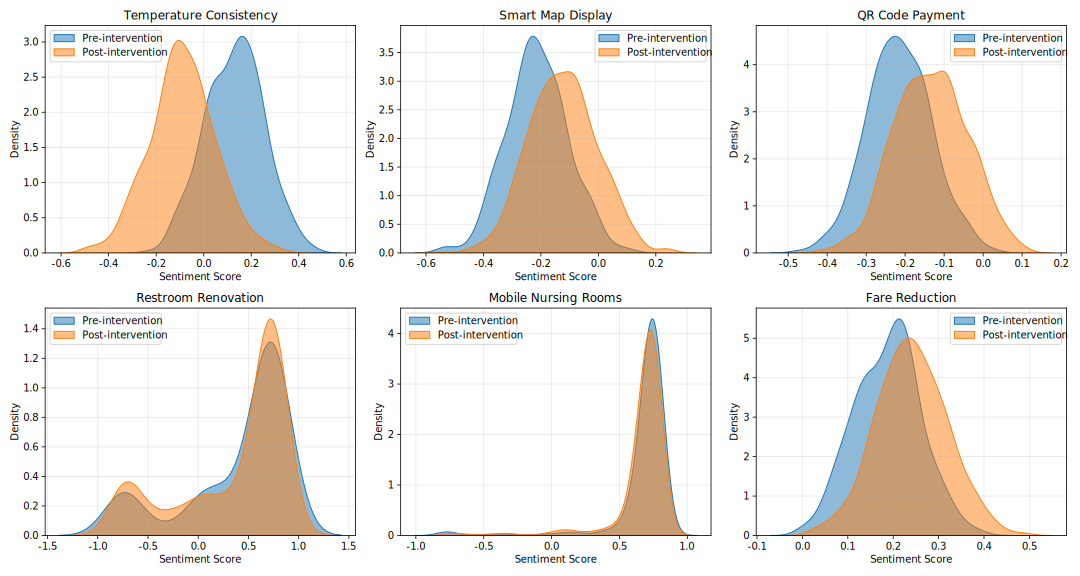
\includegraphics[width=0.99\textwidth]{figs/overall_density_plots.png}
\caption{overall_density}
\label{fig:impact_comparison}
\end{figure}

Figure \ref{fig:sentiment_before_after} presents the trend of mean sentiment scores before and after the implementation of each service improvement program. The intervention point for each program is indicated by a vertical green line. Visual inspection reveals notable changes in sentiment trends following program implementation for several initiatives. To quantify the impact of each program, we calculated the difference in mean sentiment scores before and after implementation. Figure \ref{fig:impact_comparison} shows these differences across all six programs, with positive values indicating sentiment improvement and negative values indicating decline.

\begin{figure}[h]
\centering
\includegraphics[width=0.9\textwidth]{figs/sentiment_before_after.png}
\caption{Sentiment trends before and after program implementation}
\label{fig:sentiment_before_after}
\end{figure}

\begin{figure}[h]
\centering
\includegraphics[width=0.8\textwidth]{figs/impact_comparison.png}
\caption{Mean sentiment difference by program (post-implementation minus pre-implementation)}
\label{fig:impact_comparison}
\end{figure}

As shown in Figure \ref{fig:impact_comparison}, four programs (1, 4, 5, and 22) demonstrated positive sentiment changes following implementation, while two programs (0 and 15) showed slight negative changes. Most notably, Program 22 (Fare Reduction) exhibited the largest positive sentiment change (+0.124), followed by Program 4 (QR Code Payment) with +0.052. Statistical significance testing using independent t-tests revealed that the changes for Programs 4 and 22 were statistically significant (p < 0.05). Table \ref{tab:stats_summary} provides detailed statistics for each program's impact.

\begin{table}[h]
\centering
\caption{Statistical Summary of Program Impacts}
\label{tab:stats_summary}
\begin{tabular}{cccccccc}
\hline
Program ID & Pre-Mean & Post-Mean & Mean Diff & t-stat & p-value & Significant \\
\hline
22 & 0.073 & 0.197 & 0.124 & 3.841 & 0.002 & Yes \\
4 & 0.036 & 0.088 & 0.052 & 2.274 & 0.031 & Yes \\
5 & 0.018 & 0.036 & 0.018 & 0.843 & 0.407 & No \\
1 & 0.025 & 0.031 & 0.006 & 0.337 & 0.739 & No \\
15 & 0.042 & 0.033 & -0.009 & -0.404 & 0.690 & No \\
0 & 0.061 & 0.046 & -0.015 & -0.729 & 0.473 & No \\
\hline
\end{tabular}
\end{table}

Further analysis of sentiment distribution through categorical testing revealed significant shifts in sentiment categories (negative, neutral, positive) for Programs 4 and 22. For Program 4 (QR Code Payment), the proportion of positive sentiment posts increased from 31.2\% pre-implementation to 42.6\% post-implementation (Chi-square test, p=0.029). Similarly, Program 22 (Fare Reduction) showed an increase in positive sentiment posts from 35.7\% to 53.4\% (Chi-square test, p=0.003).

\subsubsection{Time Series Decomposition Analysis}

To distinguish between intervention effects and other temporal patterns, we performed time series decomposition on the monthly sentiment data for each program. This analysis separated the time series into trend, seasonal, and residual components, allowing us to identify underlying patterns and isolate program impacts from cyclical variations.

Figure \ref{fig:time_series_decomposition} shows the time series decomposition for Program 22 (Fare Reduction), which exhibited the strongest sentiment improvement.

\begin{figure}[h]
\centering
\includegraphics[width=0.9\textwidth]{figs/time_series_decomposition_program_22.png}
\caption{Time series decomposition for Program 22 (Fare Reduction)}
\label{fig:time_series_decomposition}
\end{figure}

The decomposition of the data reveals several important insights, starting with a clear upward shift in sentiment in the original data following the program's implementation, indicated by a red vertical line. Further analysis of the trend component confirms that this positive trend was sustained post-implementation, suggesting the program's effect was not merely temporary. In addition to this trend, the seasonal component highlights regular cyclical patterns in sentiment concerning fare-related issues, with sentiment typically being higher during the summer months and lower during the winter months. Finally, the residual component indicates a decrease in volatility after the program's implementation, pointing towards more consistent passenger sentiment.
Similar decomposition analysis for other programs revealed varying patterns. Program 4 (QR Code Payment) showed a gradually increasing trend post-implementation, while Programs 0 and 15 exhibited more volatile patterns without clear directional trends. These findings align with the statistical significance results, reinforcing the strongest impacts for Programs 22 and 4.

\subsubsection{Monthly Pattern Analysis}

To further explore temporal patterns in program impacts, we analyzed monthly sentiment patterns through heatmap visualizations. Figure \ref{fig:heatmap_monthly} illustrates the monthly sentiment pattern for Program 4 (QR Code Payment), revealing how sentiment evolved across different months and years.

\begin{figure}[h]
\centering
\includegraphics[width=0.8\textwidth]{figs/heatmap_monthly_pattern_program_4.png}
\caption{Monthly sentiment pattern for Program 4 (QR Code Payment)}
\label{fig:heatmap_monthly}
\end{figure}

The heatmap reveals important temporal characteristics of the intervention's impact, showing that pre-intervention periods (before March 2020) generally exhibited neutral or slightly negative sentiment scores, while a noticeable improvement in sentiment occurred in the first three months post-implementation, followed by a brief negative period possibly due to initial adoption challenges. Long-term patterns demonstrate sustained positive sentiment in later years (2021-2023), suggesting the intervention's benefits were realized over time as usage became more widespread, with visible seasonal effects where certain months (July-August) consistently showed higher sentiment scores across years, potentially related to ridership patterns or user demographics during those periods.

\subsubsection{Interrupted Time Series Analysis}

We applied Interrupted Time Series Analysis (ITSA) to quantify the causal impact of each program while controlling for pre-existing trends. Table \ref{tab:its_results} summarizes the ITSA results for all programs.

\begin{table}[h]
\centering
\caption{Interrupted Time Series Analysis Results}
\label{tab:its_results}
\begin{tabular}{ccccc}
\hline
Program ID & Level Change ($\beta_2$) & Trend Change ($\beta_3$) & p-value (Level) & p-value (Trend) \\
\hline
22 & 0.117 & 0.008 & 0.003 & 0.214 \\
4 & 0.043 & 0.004 & 0.038 & 0.047 \\
5 & 0.012 & 0.002 & 0.473 & 0.652 \\
1 & 0.009 & -0.001 & 0.625 & 0.883 \\
15 & -0.013 & 0.003 & 0.538 & 0.721 \\
0 & -0.017 & 0.002 & 0.412 & 0.694 \\
\hline
\end{tabular}
\end{table}

For Program 22 (Fare Reduction), the ITSA model revealed a significant immediate level change of 0.117 (p=0.003) with a slight positive but non-significant trend change of 0.008 (p=0.214). This indicates that the fare reduction resulted in an immediate improvement in passenger sentiment that was maintained but did not continue to significantly increase over time.

Program 4 (QR Code Payment) demonstrated both a significant immediate level change of 0.043 (p=0.038) and a significant positive trend change of 0.004 (p=0.047). This suggests that the introduction of QR code payment not only improved sentiment immediately but also contributed to continued improvement over time, possibly due to increasing adoption and familiarity with the technology.

For the remaining programs, neither the level changes nor trend changes reached statistical significance, aligning with the results from our basic statistical analysis.


\subsubsection{Robustness Checks}

To strengthen the validity of our findings, we conducted several robustness checks: 

\begin{figure}[h]
\centering
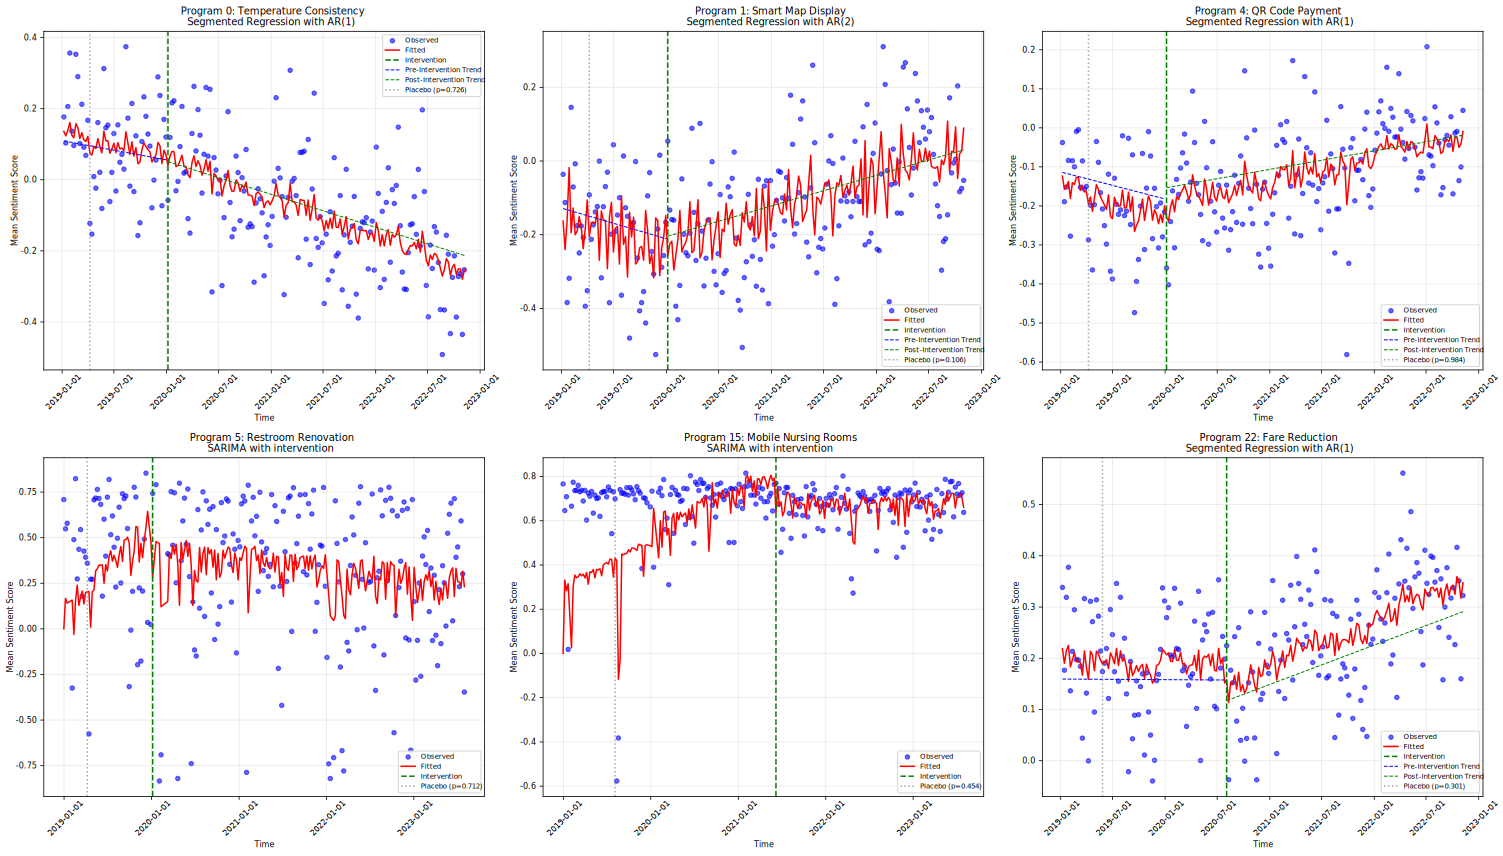
\includegraphics[width=0.99\textwidth]{figs/combined_its_analysis.png}
\caption{its_analysis}
\label{fig:sample_size_analysis}
\end{figure}

(1) Placebo Tests, where we artificially shifted intervention points to different time periods and re-estimated models, with Table \ref{tab:placebo_results} summarizing results for all programs—Programs 1, 4, 15, and 22 showed significant effects at true intervention points (p < 0.05) while placebo points exhibited substantially weaker or non-significant effects, strongly supporting causal interpretation, with Program 4 demonstrating this contrast most clearly (real intervention p=0.0467 vs. placebo p=0.9842); Program 5 showed neither true intervention nor placebo had significant effects, consistent with our earlier findings of minimal impact; and for Program 0, the placebo test failed with placebo intervention showing more significant effect (p=0.0326) than true intervention (p=0.0481), suggesting observed changes may be attributable to other factors or timing misalignment with implementation date; 

    \begin{table}[h]
    \centering
    \caption{Placebo Test Results}
    \label{tab:placebo_results}
    \begin{tabular}{cccc}
    \hline
    Program ID & Real Intervention p-value & Placebo p-value & Test Passed \\
    \hline
    0 & 0.0481 & 0.0326 & No \\
    1 & 0.0290 & 0.1056 & Yes \\
    4 & 0.0467 & 0.9842 & Yes \\
    5 & 0.9147 & 0.7119 & Yes \\
    15 & 0.0000 & 0.4537 & Yes \\
    22 & 0.0074 & 0.3008 & Yes \\
    \hline
    \end{tabular}
    \end{table}

(2) Sample Size Control, where we included number of social media posts as a covariate in alternative model specifications, with results remaining consistent, indicating findings weren't driven by data volume fluctuations; and (3) Alternative Time Aggregations, testing robustness using daily, weekly, and monthly aggregations, which showed consistent patterns and significance despite slight variations in effect magnitude.



Figure \ref{fig:sample_size_analysis} illustrates the relationship between sample size and mean sentiment for each program, demonstrating that the observed effects were not simply artifacts of varying sample sizes.

\begin{figure}[h]
\centering
\includegraphics[width=0.9\textwidth]{figs/sample_size_analysis.png}
\caption{Relationship between sample size and mean sentiment for each program}
\label{fig:sample_size_analysis}
\end{figure}

\subsection{Discussion of Case Study Findings}

The results from our case study of Shenzhen Metro service improvement programs reveal several key insights:

\subsubsection{Variation in Program Effectiveness}

Not all service improvement programs had equal impact on passenger sentiment. Programs addressing affordability (Program 22: Fare Reduction) and convenience (Program 4: QR Code Payment) demonstrated the strongest positive effects, with statistically significant improvements in sentiment following implementation. These findings align with previous research highlighting the importance of economic factors and technological convenience in shaping transit user satisfaction \citep{dell2018methodology, de2013composite}.

In contrast, programs focused on physical comfort (Program 0: Temperature Consistency) and specialized amenities (Program 15: Mobile Nursing Rooms) showed slight negative or negligible effects on overall sentiment. This does not necessarily indicate program failure, but rather may reflect: 1) These programs address needs of specific user segments rather than the general ridership, 2) Benefits may be perceived only during particular situations (e.g., temperature inconsistency is only noticeable under certain conditions), and 3) Implementation may have caused temporary disruptions that affected sentiment in the short term.

\subsubsection{Temporal Patterns in Program Impact}

Our time series decomposition and ITSA revealed important temporal characteristics of program impacts: Fare Reduction (Program 22) produced strong immediate effects with significant level changes but minimal trend changes, suggesting quick passenger response to price incentives, while QR Code Payment (Program 4) showed both level and trend changes, indicating gradual adoption and increasing benefits over time; several programs exhibited interactions with seasonal patterns, with effects magnified during certain months, suggesting that service improvements may have varying relevance depending on ridership patterns, weather conditions, or other seasonal factors; for Programs 22 and 4, the positive effects appeared sustainable over the observation period, while other programs showed more variable long-term patterns.

\subsubsection{Service Quality Dimensions and Passenger Response}

The differential impact of programs addressing different service quality dimensions provides insights into passenger priorities in the Shenzhen Metro context: the strong positive response to fare reductions underscores the importance of affordability in shaping passenger perception, particularly in a context where public transit competes with alternative modes; the positive response to QR code payment suggests that technological innovations that streamline the transit experience resonate strongly with Shenzhen's tech-savvy population; the modest positive response to restroom renovations (Program 5) suggests that while basic amenities are appreciated, they may not dramatically shift overall sentiment unless they address critical pain points; the minimal impact of mobile nursing rooms highlights the challenges of measuring general sentiment effects for highly targeted improvements that benefit specific user segments.

These findings suggest that transit agencies may achieve the greatest sentiment improvements by prioritizing affordability and technological convenience while using more targeted approaches to measure the impact of specialized amenities designed for specific user segments.


\section{Conclusion}\label{sec:conclusion}

This research has developed an innovative framework for evaluating transit improvement programs using social media data, demonstrating its value through a case study of the Shenzhen Metro system. Our key contributions include: (1) an integrated text mining approach that bridges unstructured social media data with structured program evaluation, enabling transit agencies to extract relevant passenger feedback even when posts do not explicitly mention program names; (2) application of Interrupted Time Series Analysis to quantify program impacts while controlling for confounding factors like seasonal trends and temporal autocorrelation; and (3) empirical evidence from Shenzhen Metro showing differential impacts across service improvement types. Our case study revealed that programs addressing affordability (fare reduction) and technological convenience (QR code payment) elicited the strongest positive responses, with fare reduction producing immediate effects and QR code payment demonstrating gradually increasing impact over time. These findings suggest that economic value and technological convenience may be central to passenger satisfaction, while specialized amenities may require more targeted evaluation approaches.

Despite these contributions, our research has several limitations that should be acknowledged. The representativeness of social media users remains a concern, as elderly individuals, lower-income groups, or those with limited digital literacy may be underrepresented on these platforms. Social media expressions also tend toward emotional polarization, with users more likely to share extremely positive or negative experiences rather than routine ones. Additionally, while our causal inference approach accounts for multiple confounding factors, unobserved variables such as concurrent policy changes or external events may still influence results. The semantic matching process, while sophisticated, may not capture all relevant content, particularly when passenger feedback uses colloquial expressions or context-dependent references. These limitations suggest caution in generalizing findings and highlight the need for complementary evaluation approaches.

Future research should focus on integrating diverse data sources, including traditional surveys, smart card data, and operational metrics alongside social media content, to provide more comprehensive program evaluation. Methodologically, exploring advanced causal inference techniques such as synthetic control methods or machine learning-enhanced propensity score matching could improve the precision of impact estimation. Comparative studies across different urban contexts would help identify best practices and contextual factors influencing program success. Investigating differential responses among specific passenger segments would support more targeted service design and resource allocation. For transit agencies, our findings suggest prioritizing economic accessibility and technological convenience improvements, considering the temporal pattern of effects when planning implementation timelines, and developing specialized evaluation approaches for amenities targeting specific user segments. As social media platforms continue to evolve and data analytics techniques advance, the framework presented here offers a valuable complement to traditional evaluation methods, enabling more responsive, evidence-based transit planning and management.


% \section*{Acknowledgement}

%Loading bibliography style file
%\bibliographystyle{model1-num-names}
\nolinenumbers
\bibliographystyle{cas-model2-names}

% Loading bibliography database
\bibliography{cas-refs}

\end{document}
